\documentclass[a4paper]{scrartcl}
\usepackage[
    typ=kl,
    klausurtyp=klassenarbeit,
    fach=Mathematik,
    lerngruppe=9/6,
    loesungen=keine
]{schule}

\usepackage{pgfplots}
\pgfplotsset{compat=newest, axis lines=middle}% siehe pgfplots-Anleitung

\author{Marcel Lehmann}
\date{\today}
\title{Allgemeine Potenzfunktion}

\usepackage{blindtext}

\begin{document}
\setzeAufgabentemplate{schule-randpunkte}
\begin{aufgabe}
    Gegeben ist folgender Graph\\
        \begin{center}
            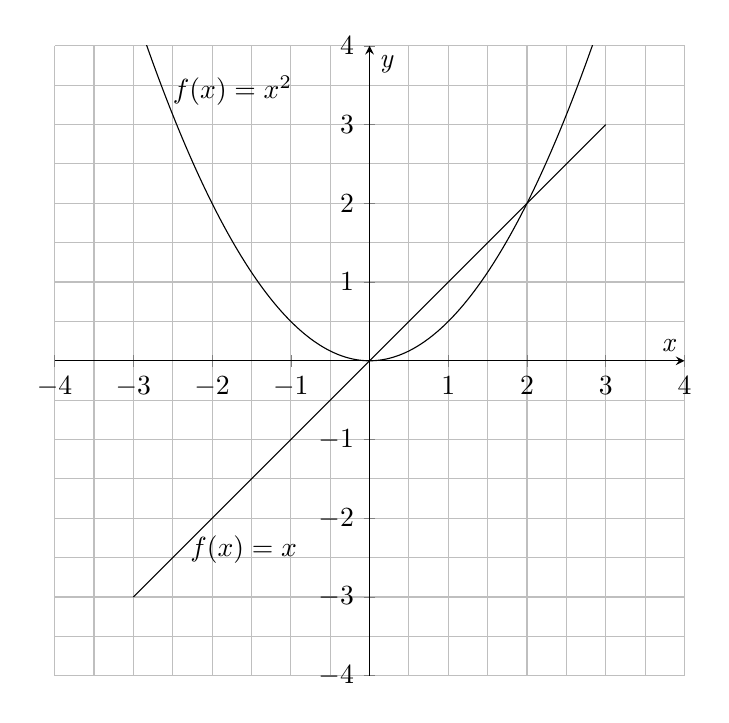
\begin{tikzpicture}
                \begin{axis}[
                    xmin=-4,xmax=4,
                    ymin=-4,ymax=4,
                    x=1cm,
                    y=1cm,
                    minor tick num=1,% zwischen zwei Haupt-Achsmarkierungen jeweils einen Untermarkierungen einfügen
                    minor tick length=0pt,% Länge der Untermarkierungen auf 0 setzen, sie also unterdrücken
                    grid={both},% Gitterlinien sowohl durch die Positionen der Haupt- als auch Untermarkierungen
                    xlabel={x}, %x-achsenbeschriftung (BITTE NICHT DEN MATHEMODUS MISSBRAUCHEN)
                    ylabel={y}, %y-achsenbeschriftung (BITTE NICHT DEN MATHEMODUS MISSBRAUCHEN)
                    label style={font=\itshape}% Achsenbeschriftung kursiv
                    ]
                    \addplot[domain=-3:3] {x}  node[right,pos=0.1]{$f(x)=x$};% Lineare Funktion
                    \addplot[domain=-3:3,samples=1000] {0.5*x^2} node[right,pos=0.1]{$f(x)=x^{2}$};% Quadratische Funktion

                \end{axis}
                \end{tikzpicture}
        \end{center}
    \begin{teilaufgaben}
    \teilaufgabe[3] Nenne....\\\\
    \begin{tikzpicture}
        \draw (2, 0) rectangle (17, 2); % Rechteck
    \end{tikzpicture}
    \teilaufgabe[2] Beschreibe....
    \teilaufgabe[1] Vergleiche...
    \end{teilaufgaben}
\end{aufgabe}
\begin{aufgabe}
Gegeben ist folgende Funktion
$$f(x)=\frac{1}{2}(x+1)^{-2}+1$$
 \begin{teilaufgaben}
  \teilaufgabe[2] Nenne...
  \teilaufgabe[3] Beschreibe..
 \end{teilaufgaben}
\end{aufgabe}

%\punktuebersicht

\end{document}
